\documentclass[a4paper]{article}
\usepackage[utf8]{inputenc}
\usepackage{polski}
\usepackage{graphicx}
\usepackage{float}
\usepackage{geometry}
\usepackage{hyperref}
\usepackage{listings}
\usepackage{xcolor}
\usepackage{minted}
\usepackage{titlepic}
\colorlet{mygray}{black!30}
\colorlet{mygreen}{green!60!blue}
\colorlet{mymauve}{red!60!blue}

\lstset{
  backgroundcolor=\color{gray!02},  
  basicstyle=\rmfamily,
  columns=fullflexible,
  breakatwhitespace=false,      
  breaklines=true,                
  captionpos=b,                    
  commentstyle=\color{mygreen}, 
  extendedchars=true,              
  frame=single,                   
  keepspaces=true,             
  keywordstyle=\color{blue},      
  language=c++,                 
  numbers=none,                
  numbersep=5pt,                   
  numberstyle=\tiny\color{blue}, 
  rulecolor=\color{white},  
  showspaces=false,               
  showtabs=false,                 
  stepnumber=5,                  
  stringstyle=\color{mymauve},    
  tabsize=3,                      
  title=\lstname                
}
\hypersetup{
    colorlinks=true, 
    linktoc=all, 
    linkcolor=black, 
}
\title{Projekt z zakresu programowania}
\author{Anastasiia Ivashchenko, Milena Mucha}
\date{February 2023}
\titlepic{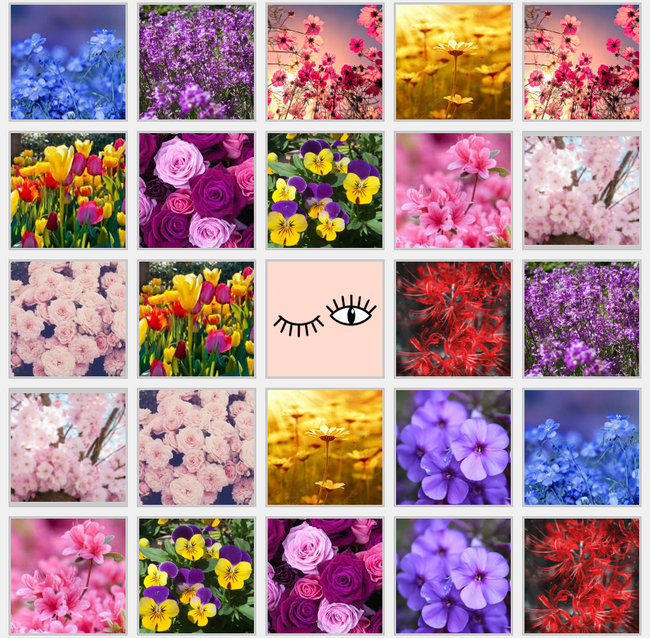
\includegraphics[width=\textwidth]{pdcz_gry2.png}}
\begin{document}
\newgeometry{tmargin=4cm, bmargin=4cm, lmargin=1.75cm, rmargin=1.75cm}
\maketitle
\newpage
\tableofcontents
\section{Opis aplikacji}
Aplikacja ,,Gra Memory" to interaktywna gra, która polega na odnajdywaniu par rysunków. Celem gry jest odnalezienie wszystkich par rysunków w jak najkrótszym czasie. Gracz klika na rysunki, aby je odsłonić i szuka par. Jeśli gracz odkryje dwa takie same rysunki, to są one zablokowane i gracz może kontynuować swoje poszukiwania. Gracz ma także opcję skorzystania z jednej ,,podpowiedzi", w której wszystkie nieodkryte rysunki są odwracane na krótki okres czasu. Aplikacja mierzy czas, w jakim gracz ukończy grę i wyświetla go na dole planszy. Jest to świetna zabawa dla osób w każdym wieku i pozwala na ćwiczenie koncentracji, zapamiętywania i logicznego myślenia.
\section{Interfejs aplikacji Memory}
Po zainstalowaniu gry Memory i po jej uruchomieniu wyświetla się okno ukazane na rysunku \ref{fig:interf}. 
\noindent
\begin{figure}[H]
    \centering
    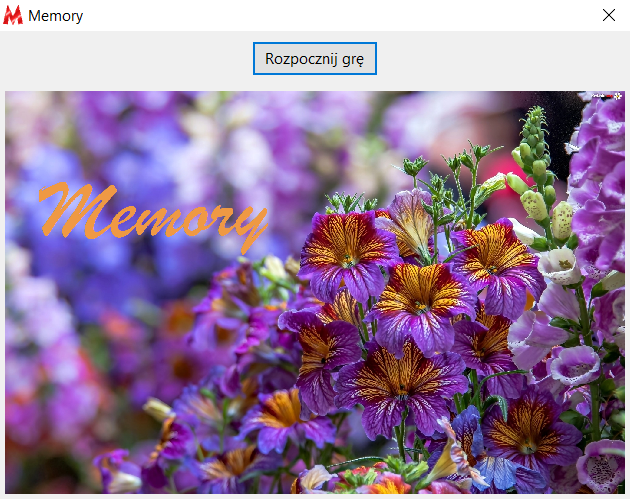
\includegraphics{interfejs.PNG}
    \caption{Interfejs gry}
    \label{fig:interf}
\end{figure}
 Po kliknięciu na przycisk ,,Rozpocznij grę" pojawia się plansza gry (patrz: Rysunek \ref{fig:plansza}).
\begin{figure}[H]
    \centering
    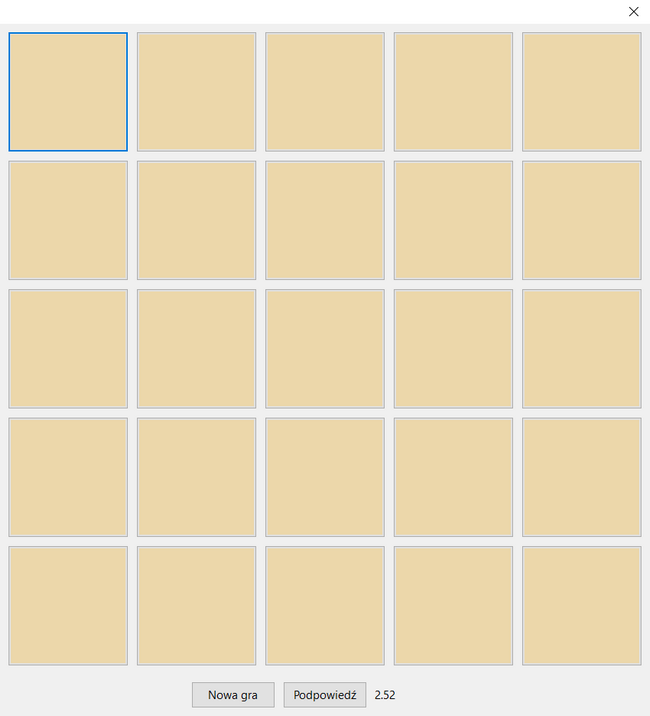
\includegraphics{plansza.PNG}
    \caption{Plansza gry}
    \label{fig:plansza}
\end{figure}
Na dole planszy znajdują się dwa przyciski: ,,Nowa gra" i ,,Podpowiedź" oraz jest liczony czas gry.
\begin{figure}[H]
    \centering
    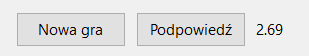
\includegraphics{przyciski.PNG}
    \caption{Przyciski na planszy}
    \label{fig:przyciski}
\end{figure}
Jeśli podczas gry została znaleziona karta, na której jest rysunek oka (patrz Rysunek \ref{fig:oko}), gracz otrzymuje podpowiedź i odpowiedni komunikat (patrz Rysunek \ref{fig:komunikat}). Może jej użyć klikając na odpowiedni przycisk. Wtedy wszystkie dotychczas nieodkryte karteczki zostaną obrócone na sekundę.
\begin{figure}[H]
    \centering
    
\includegraphics{oko.png}
    \caption{Karta z podpowiedzią}
    \label{fig:oko}
\end{figure}
\begin{figure}[H]
    \centering
    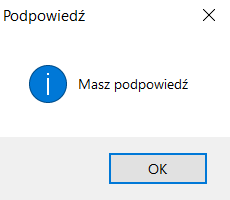
\includegraphics{podp.PNG}
    \caption{Komunikat o uzyskanej podpowiedzi}
    \label{fig:komunikat}
\end{figure}
\section{Działanie programu}
\subsection{Zmienne}
W funkcji zostały zdefiniowane następujące zmienne: 

\begin{minted}{c++}
DECLARE_EVENT_TABLE()
		wxBitmapButton * plansza[25];
        map <int,int> przelicz;
        wxBitmap rysunki[14];
        int tablica_numerow_rysunkow[25];
        wxBitmap miejsce_na_rysunek[25];
        int tablica[25] = {0,0,0,0,0,0,0,0,0,0,0,0,0,0,0,0,0,0,0,0,0,0,0,0,0};
        void funkcja_ustawiajaca_obrazki();
        void funkcja_spr_czy_rysunki_sa_takie_same(int numer);
        vector<int> wektor;
        int wygrana=0;
        int oko = 0;
        int timer = 0;
        int ile_razy_timer = 10;
\end{minted}
\subsection{Funkcja NewDialogMemory()}
\begin{minted}{c++}
#define a(nr) plansza[nr-1] = BitmapButton ## nr;
    a(1) a(2) a(3) a(4) a(5) a(6) a(7) a(8) a(9) a(10) a(11) a(12) a(13) a(14)
    a(15) a(16) a(17) a(18) a(19) a(20) a(21) a(22) a(23) a(24) a(25)
    #undef a

    rysunki[0]=wxBitmap(wxImage(_T("kremowe_tlo.bmp")));
    rysunki[1]=wxBitmap(wxImage(_T("Kwiatki1.bmp")));
    rysunki[2]=wxBitmap(wxImage(_T("Kwiatki2.bmp")));
    rysunki[3]=wxBitmap(wxImage(_T("Kwiatki3.bmp")));
    rysunki[4]=wxBitmap(wxImage(_T("Kwiatki4.bmp")));
    rysunki[5]=wxBitmap(wxImage(_T("Kwiatki5.bmp")));
    rysunki[6]=wxBitmap(wxImage(_T("Kwiatki6.bmp")));
    rysunki[7]=wxBitmap(wxImage(_T("Kwiatki7.bmp")));
    rysunki[8]=wxBitmap(wxImage(_T("Kwiatki8.bmp")));
    rysunki[9]=wxBitmap(wxImage(_T("Kwiatki9.bmp")));
    rysunki[10]=wxBitmap(wxImage(_T("Kwiatki10.bmp")));
    rysunki[11]=wxBitmap(wxImage(_T("Kwiatki11.bmp")));
    rysunki[12]=wxBitmap(wxImage(_T("Kwiatki12.bmp")));
    rysunki[13]=wxBitmap(wxImage(_T("Oko.bmp")));

    SetIcon(wxICON(aaaa));
\end{minted}
Przedstawiony fragment kodu tworzy makro, które umożliwia przypisywanie zmiennych typu BitmapButton do elementów tablicy \emph{plansza} oraz przyporządkowuje wykorzystywane w grze obrazki do tablicy \emph{rysunki}. Komenda \emph{SetIcon(wxICON(aaaa))} zmienia nam ikonę aplikacji. 
\begin{minted}{c++}
for (int i =0; i<25; i++)
    {
        plansza[i] -> SetBitmap(wxBitmap(wxImage(_T("kremowe_tlo.bmp"))));
        Connect( plansza[i]->GetId(), wxEVT_COMMAND_BUTTON_CLICKED,
                (wxObjectEventFunction)&NewDialogMemory::OnBitmapButton1Click);
        przelicz[plansza[i]->GetId()] = i;
        plansza[i]->SetBitmap(rysunki[0]);
    }
    this->Fit();
    Timer2.Start();
    funkcja_ustawiajaca_obrazki();
\end{minted}
W tym fragmencie kodu następuje ustawianie tła dla wszystkich pól w grze Memory. Dla każdego pola w pętli for, od 0 do 24, wywoływana jest funkcja SetBitmap(), która ustawia obrazek kremowego tła na danym polu. Następnie dla każdego pola łączymy jego identyfikator z funkcją OnBitmapButton1Click(), która jest wywoływana po naciśnięciu danego pola. Dla zmiennej przelicz[plansza[i]$->$GetId()] przypisujemy wartość i, aby później móc łatwo identyfikować, które pole zostało naciśnięte. Na koniec, dla każdego pola ustawiamy obrazek z tablicy rysunki[0] (Kremowe tło). 

Funkcja \emph{Fit()} ustawia wielkość okna na optymalną wielkość dla zawartości. Rozpoczyna się działanie Timer2, który odpowiada za liczenie czasu gry, oraz zostaje wywołana funkcja ustawiająca obrazki.  
\subsection{Funkcja ustawiająca obrazki}
\begin{minted}{c++}
void NewDialogMemory::funkcja_ustawiajaca_obrazki(){

    default_random_engine generator(time(0));
    uniform_int_distribution<> losowanie(0, 24);

        for(int i=1;i<=12;i++)
    {
        int liczba_wylosowana1=losowanie(generator);
        int liczba_wylosowana2=losowanie(generator);

        while(tablica[liczba_wylosowana1]!=0)
        {
            liczba_wylosowana1=losowanie(generator);
        }

        tablica[liczba_wylosowana1]=1;
        miejsce_na_rysunek[liczba_wylosowana1]=rysunki[i];
        tablica_numerow_rysunkow[liczba_wylosowana1] = i;

        while(tablica[liczba_wylosowana2]!=0)
        {
            liczba_wylosowana2=losowanie(generator);
        }
        tablica[liczba_wylosowana2]=1;
        miejsce_na_rysunek[liczba_wylosowana2]=rysunki[i];
        tablica_numerow_rysunkow[liczba_wylosowana2] = i;
    }
    for(int i=0;i<=24;i++)
    {
        if(tablica[i]==0)
        {
            miejsce_na_rysunek[i]=rysunki[13];
            tablica_numerow_rysunkow[i] = 13;
        }
    }
}
\end{minted}
W pierwszej pętli \emph{for()}, od 1 do 12, losujemy dwie liczby z przedziału od 0 do 24 za pomocą generatora losowania. W celu uniknięcia powtórzeń, sprawdza, czy dany element nie jest już zajęty, i w przypadku, gdy jest zajęty, losuje liczbę ponownie. Gdy znaleziono wolne miejsce, elementowi o indeksie \emph{liczba\textunderscore wylosowana1} przypisywana jest wartość 1, aby oznaczyć, że miejsce jest już zajęte. Dalej, odpowiadającemu temu miejscu w tablicy \emph{miejsce\textunderscore na\textunderscore rysunek} przypisywany jest i-ty rysunek, a w tablicy \emph{tablica\textunderscore numerow\textunderscore rysunków} przypisywana jest wartość i. Takie same działania wykonywane są dla drugiej liczby.

W drugiej pętli \emph{for()}, od 0 do 24, kod szuka miejsca, które jest wolne i przypisuje mu rysunek ,,oko", a odpowiadającemu temu miejscu w tablicy \emph{tablica\textunderscore numerow\textunderscore rysunków} przypisywana jest wartość 13.


\subsection{Funkcja OnBitmapButton1Click()}
\begin{minted}{c++}
void NewDialogMemory::OnBitmapButton1Click(wxCommandEvent& event)
{
    int id = event.GetId();
    int numer = przelicz[id];
    plansza[numer] -> SetBitmap(rysunki[tablica_numerow_rysunkow[numer]]);
    funkcja_spr_czy_rysunki_sa_takie_same(numer);
}
\end{minted}
Kod reaguje na kliknięcie w przycisk i pobiera jego identyfikator. Następnie tworzy nową zmienną \emph{numer}, która zapamiętuje numery klikniętych obrazków. Tło zmienia się na odpowiadający temu miejscu wcześniej przypisany obrazek kwiatu oraz wywołana zostaje funkcja, która sprawdza czy dwa kliknięte obrazki są takie same.
\subsection{Funkcja sprawdzająca czy rysunki są takie same}
\begin{minted}{c++}
void NewDialogMemory::funkcja_spr_czy_rysunki_sa_takie_same(int numer)
{
    plansza[numer]->SetBitmapDisabled(miejsce_na_rysunek[numer]);
    plansza[numer]->Enable(false);
    wektor.push_back(numer);
    if(tablica_numerow_rysunkow[wektor[wektor.size()-1]]==13 && wektor.size()%2 != 0)
    {
        Sleep(500);
        wxMessageBox(_("Masz podpowiedź"), _("Podpowiedź"));
        wygrana=wygrana+1;
        wektor.push_back(0);
        oko=1;
    }
    else if((wektor.size()%2 == 0) && tablica_numerow_rysunkow[wektor[wektor.size()-1]]==13)
    {
        Sleep(500);
        plansza[wektor[wektor.size()-2]]->Enable(true);
        plansza[wektor[wektor.size()-2]]->SetBitmap(rysunki[0]);
        wxMessageBox(_("Masz podpowiedź"), _("Podpowiedź"));
        wygrana=wygrana+1;
        oko=1;
    }
    else if((wektor.size()%2 == 0) && (tablica_numerow_rysunkow[wektor[wektor.size()-2]]
                                       != tablica_numerow_rysunkow[wektor[wektor.size()-1]]))
    {
        Sleep(500);
        plansza[wektor[wektor.size()-2]]->Enable(true);
        plansza[wektor[wektor.size()-1]]->Enable(true);
        plansza[wektor[wektor.size()-2]]->SetBitmap(rysunki[0]);
        plansza[wektor[wektor.size()-1]]->SetBitmap(rysunki[0]);
    }
    else if((wektor.size()%2 == 0) && (tablica_numerow_rysunkow[wektor[wektor.size()-2]]
                                       == tablica_numerow_rysunkow[wektor[wektor.size()-1]]))
    {
        Sleep(500);
        wygrana=wygrana+1;
    }
    if(wygrana==13)
    {
        Timer2.Stop();
        wxMessageBox(_("Wygrałeś") + (_(". Twój czas: "))+ StaticText1->GetLabel()
                     +" sekund","Koniec gry",wxICON_DEFAULT_TYPE);
        Close ();
        NewDialogMemory * dialog = new NewDialogMemory(this);
        dialog->ShowModal();
        delete dialog;
    }
}

\end{minted}
 W powyższym fragmencie kodu zostaje zablokowany obrazek, aby nie można było go już zmieniać po kliknięciu, a do wektora zostaje dodany numer klikniętego rysunku. W kodzie zdefiniowano kilka warunków, w których wykorzystywane są numery ostatniego i przedostatniego klikniętego rysunku. W zależności od sytuacji funkcja zadziała w następujący sposób:
 \begin{enumerate}
 	 \item Pierwszy wybrany obrazek okazał się okiem
\\Wyskakuje okienko z komunikatem ,,Masz podpowiedź". Na koniec wektora wstawiamy ,,0", żeby w wektorze była parzysta ilość liczb. Zmienna \emph{wygrana} zwiększa się o 1. \emph{Oko} ustawiamy na 1.

     \item Drugi wybrany obrazek okazał się okiem
\\ Program odblokowuje pierwszy zablokowany obrazek i ustawia na nim kremowe tło. Wyskakuje okienko z komunikatem ,,Masz podpowiedź". Zmienna \emph{wygrana} zwiększa się o 1. \emph{Oko} ustawiamy na 1.
     \item Obrazki nie są takie same
\\W takim przypadku, oba rysunki są odblokowywane i zamieniane na kremowe tło. 
     \item Obrazki są takie same
\\Obrazki pozostają odkryte a zmienna \emph{wygrana} zwiększa się o 1.
     \item Wartość zmiennej \emph{wygrana} jest równa 13
\\\emph{Wygrana} jest równa 13 jeśli zostały odnalezione wszystkie 12 par kart oraz oko. W takim przypadku program kończy działanie funkcji \emph{Timer2}, wyświetla komunikat o wygranej gracza zawierający czas jaki zajęła mu rozgrywka, a następnie zamyka obecną planszę i tworzy nową planszę.
 \end{enumerate}
 \subsection{Funkcja OnButton1Click1()}
\begin{minted}{c++}
void NewDialogMemory::OnButton1Click1(wxCommandEvent& event)
{
    Close ();
    NewDialogMemory * dialog = new NewDialogMemory(NULL);
    dialog->ShowModal();
    delete dialog;

}
\end{minted}
Ta funkcja jest uruchamiana przez kliknięcie przycisku ,,Nowa gra" na planszy. Po jej wywołaniu, obecna plansza jest zamknięta i wyświetlana jest nowa plansza gry, która jest tworzona jako nowy obiekt klasy ,,NewDialogMemory".  Po zakończeniu gry, obiekt ten jest usuwany z pamięci.
\subsection{Funkcja OnTimer1Trigger()}
\begin{minted}{c++}
void NewDialogMemory::OnTimer1Trigger(wxTimerEvent& event)
{
    timer++;
    if(timer == 1)
    {
        for(int i = 0; i <= 24; i++)
            plansza[i] -> SetBitmap(wxBitmap(wxImage(_T("kremowe_tlo.bmp"))));
        Timer1.Stop();
    }
}
\end{minted}
 Timer ten odpowiada za powrót obrazków na planszy do ich początkowego stanu po kliknięciu na przycisk ,,podpowiedź". Po upływie jednej sekundy, pętla for() jest uruchamiana, aby znaleźć i zakryć niezablokowane obrazki (których para jeszcze nie została odnaleziona). Po wykonaniu tej czynności, \emph{Timer1} kończy swoje działanie i plansza jest gotowa do kontynuowania gry.
 \subsection{Funkcja OnTimer2Trigger()}
\begin{minted}{c++}
void NewDialogMemory::OnTimer2Trigger(wxTimerEvent& event)
{
    ile_razy_timer=ile_razy_timer+1;
    double s = ile_razy_timer * Timer2.GetInterval()/640.0;
    StaticText1->SetLabel(wxString::Format("%.2f",s));
}
\end{minted}
Funkcja ta jest odpowiedzialna za mierzenie i wyświetlanie czasu trwania gry na planszy.
Timer2 ustawiony jest tak, aby czas, który jest wyświetlany, był jak najbardziej zgodny z rzeczywistym upływem czasu.
Funkcja używa zmiennej \emph{ile\textunderscore razy\textunderscore timer}, która jest zwiększana o jeden przy każdym wywołaniu timera, aby obliczyć łączny czas gry. Interwał timera jest wykorzystywany do obliczenia czasu w sekundach i wyświetlany jest na dole planszy za pomocą elementu ,,StaticText1".
\subsection{Funkcja OnButton2Click1()}
\begin{minted}{c++}
void NewDialogMemory::OnButton2Click1(wxCommandEvent& event)
{
    if(oko==0)
        wxMessageBox(_("Nie masz podpowiedzi"), "Brak podpowiedzi");
    else
    {
        for(int i = 0; i <= 24; i++)
        {
            plansza[i] -> SetBitmap(rysunki[tablica_numerow_rysunkow[i]]);
        }
        Timer1.Start();
        timer = 0;
        oko=0;
    }
}
\end{minted}
Ta funkcja jest jest uruchamiana po kliknięciu na przycisk ,,podpowiedź"
Jeśli rysunek z okiem jeszcze nie został znaleziony, to zostaje wyświetlony komunikat ,,Nie masz podpowiedzi". W przeciwnym przypadku funkcja odwraca wszystkie obrazki, które jeszcze nie zostały otwarte nie blokując ich. Dalej rozpoczyna się działanie Timer1, a po jego zakończeniu zmienne \emph{timer} i \emph{oko} zostają ustawione na 0. 
\section{Udział procentowy}
\begin{itemize}
    \item Pomysł: Anastasiia Ivashchenko 50\%, Milena Mucha 50\%
    \item Tworzenie planszy do gry: Anastasiia Ivashchenko 50\%, Milena Mucha 50\%
    \item Tworzenie programu: Anastasiia Ivashchenko 70\%, Milena Mucha 30\%
    \item Wygląd estetyczny i grafika: Anastasiia Ivashchenko 25\%, Milena Mucha 75\%
    \item Tworzenie dokumentacji: Anastasiia Ivashchenko 50\%, Milena Mucha 50\%
    \item Korekcja błędów programu: Anastasiia Ivashchenko 75\%, Milena Mucha 25\%
    \item Tworzenie pliku instalacyjnego: Anastasiia Ivashchenko 25\%, Milena Mucha 75\%
\end{itemize}



\end{document}
